\documentclass[10pt,a4paper,twocolumn,twoside]{article}
\usepackage[utf8]{inputenc}
\usepackage[catalan]{babel}
\usepackage{multicol}
\usepackage{graphicx}
\usepackage{fancyhdr}
\usepackage{times}
\usepackage{titlesec}
\usepackage{multirow}
\usepackage{lettrine}
\usepackage[top=2cm, bottom=1.5cm, left=2cm, right=2cm]{geometry}
\usepackage[figurename=Fig.,tablename=TAULA]{caption}
\captionsetup[table]{textfont=sc}

\author{\LARGE\sffamily Pau Casacuberta Orta}
\title{\Huge{\sffamily Disseny d'un ``core'' RISC-V Didàctc}}
\date{}

\newcommand\blfootnote[1]{%
  \begingroup
  \renewcommand\thefootnote{}\footnote{#1}%
  \addtocounter{footnote}{-1}%
  \endgroup
}

%
%\large\bfseries\sffamily
\titleformat{\section}
{\large\sffamily\scshape\bfseries}
{\textbf{\thesection}}{1em}{}

\begin{document}

\fancyhead[LO]{\scriptsize Pau Casacuberta Orta: Disseny d'un ``core'' RISC-V Didàctc}
\fancyhead[RO]{\thepage}
\fancyhead[LE]{\thepage}
\fancyhead[RE]{\scriptsize EE/UAB TFG INFORMÀTICA: Disseny d'un ``core'' RISC-V Didàctc}

\fancyfoot[CO,CE]{}

\fancypagestyle{primerapagina}
{
   \fancyhf{}
   \fancyhead[L]{\scriptsize TFG EN ENGINYERIA INFORMÀTICA, ESCOLA D'ENGINYERIA (EE), UNIVERSITAT AUTÒNOMA DE BARCELONA (UAB)}
   \fancyfoot[C]{\scriptsize Febrer de 2020, Escola d'Enginyeria (UAB)}
}

%\lhead{\thepage}
%\chead{}
%\rhead{\tiny EE/UAB TFG INFORMÀTICA: TÍTOL (ABREUJAT SI ÉS MOLT LLARG)}
%\lhead{ EE/UAB \thepage}
%\lfoot{}
%\cfoot{\tiny{February 2015, Escola d'Enginyeria (UAB)}}
%\rfoot{}
\renewcommand{\headrulewidth}{0pt}
\renewcommand{\footrulewidth}{0pt}
\pagestyle{fancy}

%\thispagestyle{myheadings}
\twocolumn[\begin{@twocolumnfalse}

%\vspace*{-1cm}{\scriptsize TFG EN ENGINYERIA INFORMÀTICA, ESCOLA D'ENGINYERIA (EE), UNIVERSITAT AUTÒNOMA DE BARCELONA (UAB)}

\maketitle

\thispagestyle{primerapagina}
%\twocolumn[\begin{@twocolumnfalse}
%\maketitle
%\begin{abstract}
\begin{center}
\parbox{0.915\textwidth}
{\sffamily
\textbf{Resum--}
Resum del projecte, màxim 10 línies. ........ ........... .......... ..  ... ..... .... ........ ........... .......... ..  ... ..... .... ........ ........... .......... ..  ... ..... .... ........ ........... .......... ..  ... ..... .... ........ ........... .......... ..  ... ..... .... ........ ........... .......... ..  ... ..... .... ........ ........... .......... ..  ... ..... .... ........ ........... .......... ..  ... ..... .... ........ ........... .......... ..  ... ..... .... ........ ........... .......... ..  ... ..... .... ........ ........... .......... ..  ... ..... .... .................. ..  ... ..... .... ........ ........... .......... ..  ... ..... .... ........ ........... .......... ..  ... ..... .... ........ ........... .......... ..  ... ..... .... ........ ........... .......... ..  ... ..... .... ........ ........... .......... ..  ... ..... .... ........ ........ .......... ..  ... . ........... .......... ..  ... ..... .... ........ ........... .......... ..  ... ..... .... ........ ........... .......... ..  ... ..... .... ........ ........... .......... ..  ... ........... ..  ... ..... .... ........ ........... .......... ..  ... ..... .... ........ ........... .......... ..  ... ..... .... ........ ........... .......... ..  ... ..... .... ........ ........... .......... ..  ... ..... .... ........ ........... .......... ..  ... ..... .... ........ ........... .......... ..  ... ..... .... ........ ........... .......... ..  ... ..... .... ........ ........... .......... ..  ... ..... .... 
\\
\\
\textbf{Paraules clau-- } Paraules clau del treball, màxim 2 línies . .... ........ ........... .......... ..  ... ..... .... ........ ........... .......... ..  ... ..... .... ........ ........... ................\\
\\
%\end{abstract}
%\bigskip
%\begin{abstract}
\bigskip
\\
\textbf{Abstract--} Versió en anglès del resum . ........ ........... .......... ..  ... ..... .... ........ ........... .......... ..  ... ..... .... ........ ........... .......... ..  ... ..... .... ........ ........... .......... ..  ... ..... .... ........ ........... .......... ..  ... ..... .... ........ ........... .......... ..  ... ..... .... ........ ........... .......... ..  ... ..... .... ........ ........... .......... ..  ... ..... .... ........ ........... .......... ..  ... ..... .... ........ ........... .......... ..  ... ..... .... ........ ........... .......... ..  ... ..... .... .................. ..  ... ..... .... ........ ........... .......... ..  ... ..... .... ........ ........... .......... ..  ... ..... .... ........ ........... .......... ..  ... ..... .... ........ ........... .......... ..  ... ..... .... ........ ........... .......... ..  ... ..... .... ........ ........ .......... ..  ... . ........... .......... ..  ... ..... .... ........ ........... .......... ..  ... ..... .... ........ ........... .......... ..  ... ..... .... ........ ........... .......... ..  ... ........... ..  ... ..... .... ........ ........... .......... ..  ... ..... .... ........ ........... .......... ..  ... ..... .... ........ ........... .......... ..  ... ..... .... ........ ........... .......... ..  ... ..... .... ........ ........... .......... ..  ... ..... .... ........ ........... .......... ..  ... ..... .... ........ ........... .......... ..  ... ..... .... ........ ........... .......... ..  ... ..... .... 
\\
\\
\textbf{Keywords-- } Versió en anglès de les paraules clau. .... ........ ........... .......... ..  ... ..... .... ........ ........... .......... ..  ... ..... .... ........ ........... .................. ..\\
}

\bigskip

{\vrule depth 0pt height 0.5pt width 4cm\hspace{7.5pt}%
\raisebox{-3.5pt}{\fontfamily{pzd}\fontencoding{U}\fontseries{m}\fontshape{n}\fontsize{11}{12}\selectfont\char70}%
\hspace{7.5pt}\vrule depth 0pt height 0.5pt width 4cm\relax}

\end{center}

\bigskip
%\end{abstract}
\end{@twocolumnfalse}]

\blfootnote{$\bullet$ E-mail de contacte: pau.casacubertao@e-campus.uab.cat}
\blfootnote{$\bullet$ Menció realitzada: Enginyeria de Computadors }
\blfootnote{$\bullet$ Treball tutoritzat per: nom i cognoms del tutor (departament)}
\blfootnote{$\bullet$ Curs 2019/20}

\section{Introducció}
%Secció d’introducció on es motiva el treball i es plantegen els objectius, i també s’explica breument l’organització de la resta del document.
\lettrine[lines=3]{E}{n} el disseny d'arquitectures de computadors la part més important a l'hora de construir aquest és l'elecció d'un conjunt d'instruccions que aquest podrà executar, ja que a partir de les operacions bàsiques es farà el disseny del propi nucli i dels mòduls que el conformen. 
El repertori es la manera de poder generar programes que després podrà executar el processador.  trobem dos jocs d'instruccions principals a l'hora de dissenyar processadors per a ordinadors. 
Els principals jocs d'instruccions per a processadors d'us generals (ordinadors personals i dispositius mòbils) són x86 i ARM, on cada una té dissenys diferents i si es vol utilitzar per a algun futur dispositius s'ha de llicenciar l'us.

Ara bé, per canviar aquest entorn limitat d'opcions propietàries fa uns anys ha anat creixent una iniciativa, iniciada a la Universitat de Califòrnia a Berkeley \cite{krste_asanovic_instruction_2014}, que proposa un disseny de processador obert i lliure, això ho aconsegueix alliberant el repertori d'instruccions, en anglès ISA (Instruction Set Architecture), al public. Això permet que qualsevol universitat o empresa pugui crear una arquitectura a partir d'aquest repertori lliure de royalties i amb l'opció de poder-se involucrar en el desenvolupament, iniciant un camí cap al hardware obert i lliure. 

Aquesta nova arquitectura es diu RISCV i últimament està dominant les tendències i estratègies de futur i prometen una ràpida expansió.

Aquest Treball Fi de Grau pretén proposar un disseny d'un nucli de processador RISCV amb l’objectiu d’anar avançant cap un entorn didàctic per a conèixer aquest tipus de processador, des del propi nucli del processador fins a un entorn gràfic que permeti mostrar l'execució de programes escrits en C, indicant quines parts del nucli es fan servir.
Tot això com a eina didàctica per a entendre el funcionament dels computadors amb conjunts d'instruccions actuals. 

Concretament la micro-arquitectura que s'implementarà consistirà en un subconjunt del repertori d’instruccions, el \textbf{ISA-RV32I}. 
Aquest nucli serà mono-cicle i d’execució seqüencial d’instruccions. 

A la secció \ref{sec:Obj} es detallen els objectius





\section{Objectius} 
\label{sec:Obj}
El principal objectiu d'aquest treball és produir un disseny d'un nucli RISCV a nivell RTL en Verilog on el codi sigui fàcil de seguir i provar que es funcional implementant-lo en una FPGA i executar programes compilats amb eines preparades per al repertori de RISCV.

Aquest objectiu el podem dividir en diferents sub-objectius:

\begin{itemize}

    \item Aprendre a dissenyar un computador des de zero fent recerca d'informació. Aquesta recerca es basarà en consultar els documents oficials sobre l'ISA de RISCV \cite{waterman_volume_2019} \cite{waterman_volume_2019-1}  així com altres llibres que es centren més en el disseny de nuclis de processadors \cite{patterson_computer_2018} o en el llenguatge de descripció de hardware utilitzat, en aquest cas Verilog \cite{li_implementing_2018}.
    
    \item Fer un disseny funcional de parts del nucli per verificar el funcionament amb Verilog.

    \item Especificar i dissenyar a nivell HDL-RTL un nucli RISC-V amb el subconjunt bàsic de l’ISA, el RV32I.
    
    \item Preparar un Testbench per a comprovar el funcionament del nucli.
    
    \item Proporcionar un Core de Risc-V funcional (que permeti l'execució de programes simples escrits en C) però fàcil d'entendre'n la descripció en HDL.
    
    \item Per aplicar altres coneixements de la carrera, utilitzar eines de DevOps per a automatitzar gran part de la part de tests i preparar eines per a desenvolupar el codi del processador.
    
    \item Materialitzar i testejar el nucli anterior en una placa de desenvolupament basada en FPGA.
    
        
\end{itemize}

\section{Estat del Art}
        Mostrar Cores, i aplicacions 
        
        Diversos projectes de nuclis de RISCV, molts utilitzen altres llenguatges per a obtenir l'arxiu final en verilog i poden ser més difícils de seguir que un llenguatge d'HDL.
        
        Plataformes que permeten entorn per a nuclis RISCV.
%\section{Finalitat del projecte}

\section{Core Risc-V}
A l'hora de dissenyar la micro-arquitectura del processador és important analitzar bé el repertori d'instruccions per a definir els elements que seran necessaris per a poder executar cada una d'aquestes instruccions.

A part del repertori d'instruccions qualsevol processador ha de tenir la possibilitat de poder emmagatzemar dades en \textbf{registres interns} i poder identificar cada línia de programa amb un altre registre anomenat\textbf{ Program Counter}.
En aquesta secció es descriurà en detall cada part del nucli. 
    \subsection{Instruction set}
    Per a dissenyar un nucli de processador primer s'ha de determinar quin repertori d'instruccions haurà d'executar, per aquest motiu a continuació es descriu com està composat el repertori RV32I utilitzat per al disseny del nucli en qüestió.
        \subsubsection{RV32I}
        S'ha escollit el repertori RV32I degut a que és el més simple i permet fer operacions aritmeticològiques amb nombres enters, carregar i guardar dades a memòria externa, així com salts condicionals i incondicionals dins un programa.  
        
        Per a poder analitzar el conjunt d'instruccions aquestes es poden separar segons el tipus d'instrucció.
        
        \begin{figure}[!h]
        \centering
        	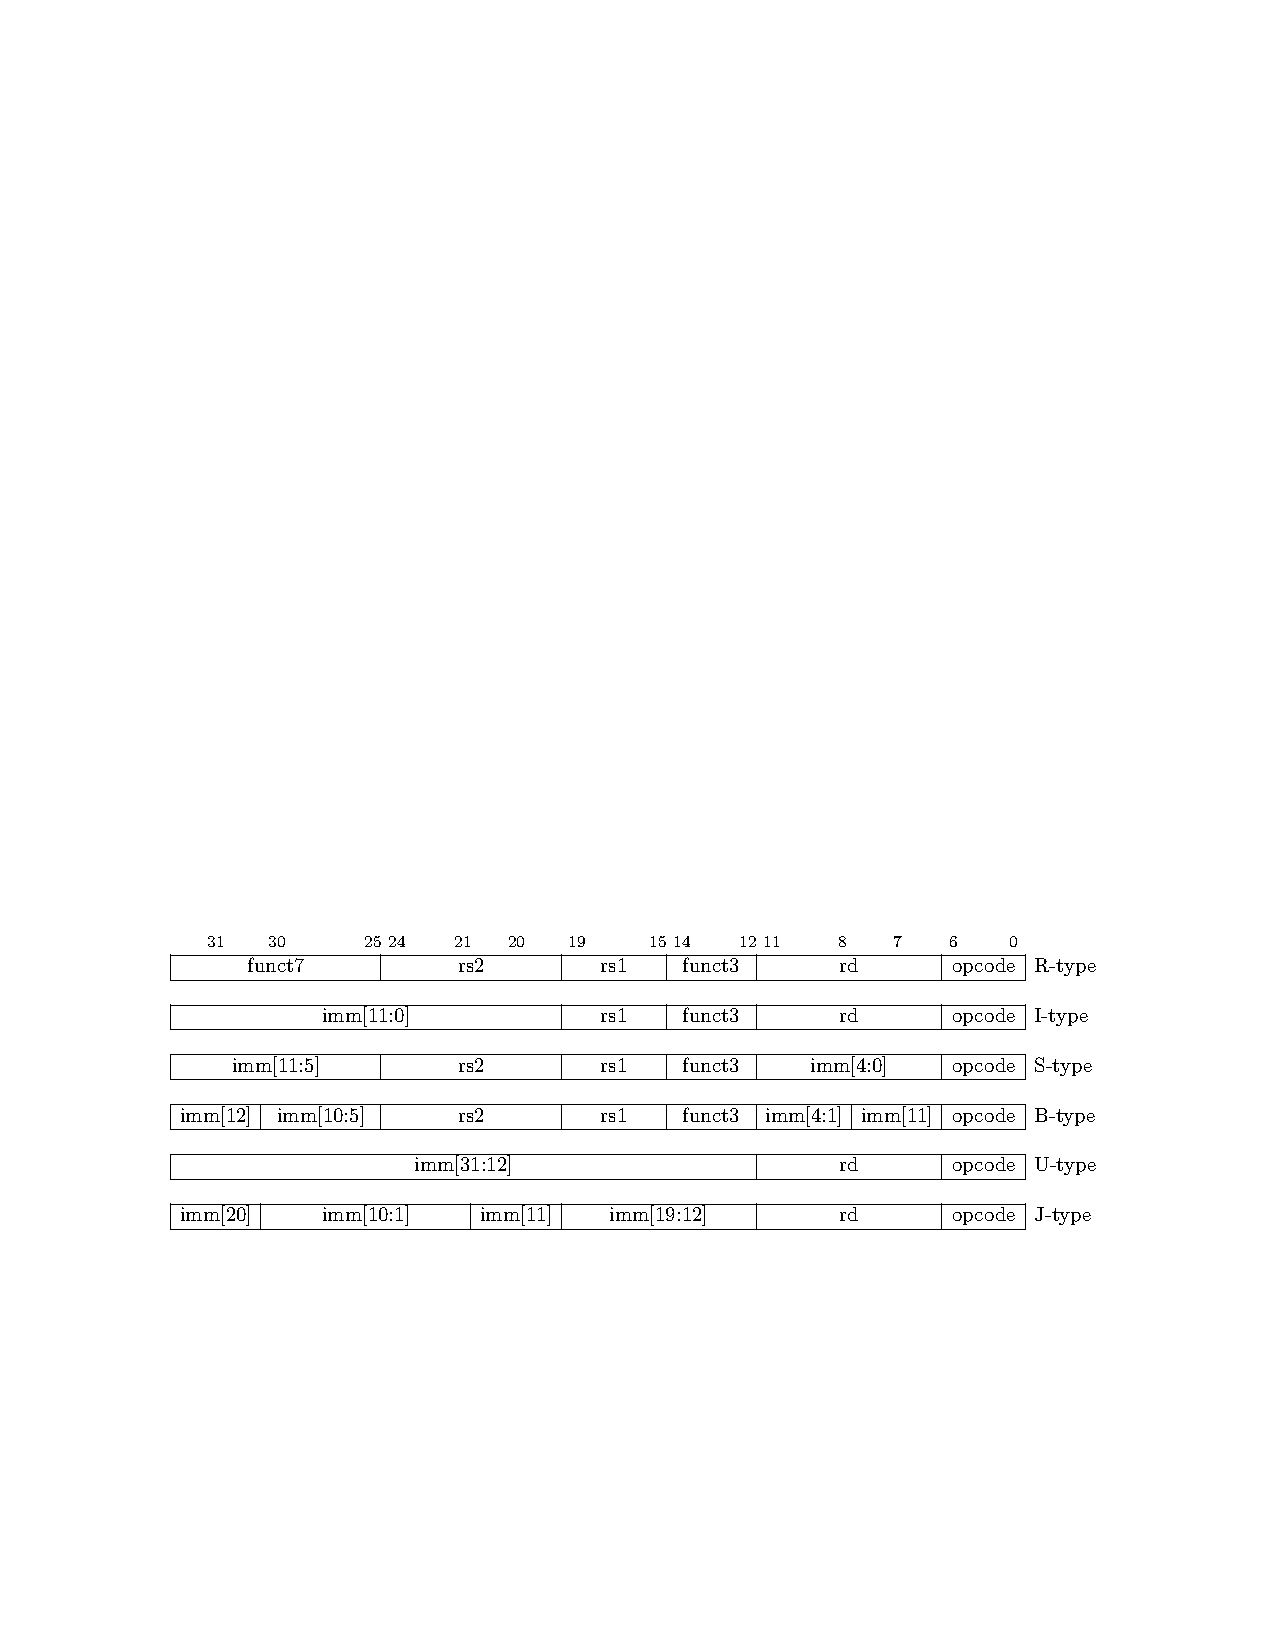
\includegraphics[width=\linewidth]{pdf/Encoding.pdf}
            \caption{RISC-V base instruction formats showing immediate variants.}
            \label{fig:baseinstformatsimm}
        \end{figure}
        
        En aquest proces de disseny s'ha decidit dividir les instruccions en quatre grups segons l'acció que s'efectua:
        
        \begin{itemize}
            \item Aritmeticològiques. Operacions que utilitzen valors instantanis o guardats en registres per a aplicar una operació aritmeticològica i guardar el resultat en un registre del banc de registres.
            \item Lectura o escriptura de dades a memòria externa. Operacions que a partir d'una adreça de memòria es guarda una dada de la memòria externa a un registre del banc de registres, o anàlogament guardar una dada d'un registre intern a una posició de memòria externa.
            \item Salts d'execució. Operacions que permeten modificar el valor del registre Comptador de Programa ja sigui després d'avaluar una comparació entre dos registres o de manera incondicional.
            \item Control del processador. Operacions relacionades amb registres d'estat i de control del processador i sistema d'interrupcions, en aquesta implementació no hi ha cap interrupció i els registres de control implementats son els mínims per complir amb l'especificació de RV32I en mode usuari.
        \end{itemize}
        
        
        
    
        
        
        
    \subsection{Arquitectura}
    En aquesta secció s'indica l'organització a alt nivell dels elements del nucli.
        \subsubsection{Unitats i blocs arquitecturals}
        Esquema de blocs general
        Esquema que mostra les unitats principals, com el comptador de programa, unitat de control, banc de registres, Unitat d'execució i dins d'aquesta les unitats de Branching, càrrega i escriptura de dades a memòria, i una unitat de CSR que conté comptadors per a obtenir informació del rendiment del propi nucli.
    \subsection{Senyals de Control}
    En aquesta secció es descriu quins senyals fan falta per a operar el core i els senyals interns que intercomuniquen les diferents unitats.
        \subsubsection{Connexions externes}
        Les senyals bàsiques per a poder operar el nucli des de l'exterior són:
        \begin{itemize}
            \item Els senyals de rellotge i reset: bàsics per a poder determinar la velocitat amb la que funcionarà aquest, és a dir cada quan els circuits seqüencials actualitzen les dades.
            \item Senyals relacionats amb les paraules de programa: conformats per un bus d'adreça (de com a molt 32 bits) que determina la posició en bytes de la següent línia de programa carregar i un altre bus (de 32 bits) que proporcionarà els 4 bytes que conformen una paraula de programa.
            \item Senyals relacionats amb la memòria de dades: conformats per un bus d'adreça (de com a molt 32 bits) que determina la posició en bytes de la dada que volem carregar o escriure, així com un bus de 4 bits que determina una màscara de quins bytes interessa modificar (per poder guardar un sol byte, mitja paraula o 2 bytes o una paraula sencera 4 bytes), també un senyal d'un bit per determinar si es vol escriure o llegir de la memòria i un altre bus (de 32 bits) que proporcionarà les dades que s'hagin d'escriure o llegir.
        \end{itemize}
        
        \subsubsection{Senyals interns}
        
        *Senyals que determinen les operacions que han de fer altres mòduls (ALU, BR, LIS), senyals que informen de salts en el programa per a que diferents mòduls actuïn en consonància, senyals que indiquen adreces per llegir o escriure al banc de registres, senyals de control d'escriptura o lectura de dades al banc de registres, senyals que informen del comptador de programa de la instrucció actual.
    
    \subsection{Unitat de Control}
    Mostrar esquema de la unitat de control 
    
    *Destacar que consta de dos parts principals, una primera part que separa la paraula de programa en els blocs que defineix la especificació de RiscV i després un sistema que tria quines senyals de control activar segons els codis d'operació.
    
    wires interns 
    gran switch case
    
    \subsection{Unitat d'execució}
    Per compartimentar millor el core, s'ha definit un bloc d'execució que engloba les unitats de càlcul aritmeticològic, d'accés a memòria, i de salts de programa.
    
    *Principalment aquesta unitat consta de dos multiplexors que determinen les dades d'entrada a les sub-unitats d'execució (ALU, BR, LIS), així com les dades de sortida que surten de dites sub-unitats i van cap al banc de registres.
    
    2 switch cases
    
    
    \subsection{Unitat Aritmetico-Lògica}
    Part principal per a executar les operacions de suma, resta, multiplicació, emmascarament, desplaçament...
    Circuit purament combinacional
    Switch case 
    \subsection{Unitat de Lectura i escriptura}
    *Unitat que gestiona les connexions amb la memòria de dades, s'encarrega de determinar els valors de la màcara de bytes i l'adreça de la dada que es vol accedir tant per a escriptura com per lectura.
    Switch case
    \subsection{ Càrrega d'instruccions i unitat de salts}%Fetch and Jumps}
    *Unitat que s'encarrega de proporcionar la seguent adreça que s'aurà de demanar a la memòria de programa tenint en compte si s'executa una operació de salt.
    
    Sumador extra
    senyal de alu = 0 per comparar
    
    \subsection{CSR}
    
    *Unitat que connecta diversos comptadors a les línies de dades internes del nucli
    
    \subsection{Nucli RISC-V complet}
    *Comentar la necessitat de tenir les dues memòries (prog + dades) separades i implementades com a bancs de registres per a no afegir latència a l'hora de llegir dades i poder executar operacions de lectura en un sol cicle de rellotge
        \subsubsection{Arquitectura}
        *Diseny bàsic per al repertori de dades
        \subsubsection{Memòria de Programa}
        *Implementació com a reg file per no haver de registrar 2 cops el PC
        \subsubsection{Memòria de Dades}
        *Implementació com a reg file per a poder llegir dades al mateix cicle que s'indica l'adreça de la dada.
        
        
\section{Core Risc-V adaptat a memòries arbitrades}
    * Degut a les decisions al apartat anterior no es pot utilitzar el core en un entorn amb memòries arbitràries, es necessari complicar lleugerament el disseny per a adaptar-lo a entorns reals.
    \subsection{Plataforma Pulpino}
    *Per a poder verificar el funcionament amb memòries externes reals s'ha decidit adaptar el nucli a una plataforma ja creada i testejada per a verificar que el funcionament és correcte.
    S'ha agafat el multiplexor que arbitra l'accés a les memòries que afegeix latència i senyals de control extres per a poder adaptar el core.
    \subsection{Modificacions necessàries}
    A continuació es mostren les modificacions necessàries per a adaptar el core
        \subsubsection{Senyals}
        Senyals externs per a demanar accés al bus de dades o de programa així com senyals que garanteixen l'accés i verificacions d'escriptura
        \subsubsection{Estats}
        Necessitat que el core sigui conscient de en quin estat està a l'hora de fer una transacció de memòria
        \subsubsection{Stall Core}
        Necessitat de parar l'execució d'el programa per a esperar noves dades mentre el bus està ocupat per una altre recurs.
        
        
\section{Del RTL a la FPGA}  % Correu1.1
Com s'ha fet la sintetizació 
    \subsection{Embolcall FPGA}
    Necesitat d'un embolcall per adaptar-lo al entorn de desenvolupament de la FPGA
    \subsection{Programació FPGA}
    Compilació, sintetizació del codi verilog i programació de la FPGA
    \subsection{Funcionament}
    Mostra de funcionament

\section{Resum de resultats (desenvolupament i test)}
% Una secció on es presenti el mètode d’avaluació dels resultats, els resultats en si mateixos, i una discussió/reflexió sobre aquests resultats.
Mostrar Testbench i resultats

\section{Metodologia}
TEcnologies utilitzades per al desenvolupament, VSC, Icarus Verilog, GitHub, Docker, GCC, Travis.
\subsection{Flux de disseny}  % Correu1.2
\section{Conclusions i treball de futur}  % Correu1.3
Apartat on es comenta el desenvolupament del projecte 

Revisar i simplificar CSR, Possible adaptació a Pipeline, debug ring...
    
    



\section*{Agraïments}

... ..  .... .. .... ... ..... ... ..... ... ... ..... .... .
.... ..  .... .. .... ... ..... ... ..... ... ... ..... .... .
.... ..  .... .. .... ... ..... ... ..... ... ... ..... .... .
.... ..  .... .. .... ... ..... ... ..... ... ... ..... .... .
.... ..  .... .. .... ... ..... ... ..... ... ... ..... .... .


\bibliographystyle{IEEEtran}
\bibliography{references.bib}

%\begin{thebibliography}{11}
%\bibitem{latex}
%http://en.wikibooks.org/wiki/LaTeX

%\bibitem{2}
%Referència 2

%\bibitem{3}
%Etc.


%\end{thebibliography}

\appendix

\section*{Apèndix}

\setcounter{section}{1}

\subsection{Secció d'Apèndix}
% Utilitzeu el begin table només en cas de vole taules flotants. Si les voleu al lloc, tabular directament.
\begin{table}[h]
\caption{Taula d'exemple}
\label{tab:senzilla}
\begin{center}
\begin{tabular}{|c|c|}
\hline
One & Two\\
\hline
Three & Four\\
\hline
\end{tabular}
\end{center}
\end{table}

... ..  .... .. .... ... ..... ... ..... ... ... ..... .... .
.... ..  .... .. .... ... ..... ... ..... ... ... ..... .... .
.... ..  .... .. .... ... ..... ... ..... ... ... ..... .... .
.... ..  .... .. .... ... ..... ... ..... ... ... ..... .... .
.... ..  .... .. .... ... ..... ... ..... ... ... ..... .... .

\subsection{Secció d'Apèndix}


... ..  .... .. .... ... ..... ... ..... ... ... ..... .... .
.... ..  .... .. .... ... ..... ... ..... ... ... ..... .... .
.... ..  .... .. .... ... ..... ... ..... ... ... ..... .... .
.... ..  .... .. .... ... ..... ... ..... ... ... ..... .... .
.... ..  .... .. .... ... ..... ... ..... ... ... ..... .... .


\end{document}

